\documentclass[pscyr,specification,annotation]{itmo-student-thesis}

%% Опции пакета:
%% - specification - если есть, генерируется задание, иначе не генерируется
%% - annotation - если есть, генерируется аннотация, иначе не генерируется
%% - times - делает все шрифтом Times New Roman, собирается с помощью xelatex
%% - pscyr - делает все шрифтом Times New Roman, требует пакета pscyr.

\usepackage{graphicx}
\graphicspath{{logo/}{pics/}}

%% Делает запятую в формулах более интеллектуальной, например:
%% $1,5x$ будет читаться как полтора икса, а не один запятая пять иксов.
%% Однако если написать $1, 5x$, то все будет как прежде.
\usepackage{icomma}

%% Один из пакетов, позволяющий делать таблицы на всю ширину текста.
\usepackage{tabularx}

%% Данные пакеты необязательны к использованию в бакалаврских/магистерских
%% Они нужны для иллюстративных целей
%% Начало
\usepackage{tikz}
\usetikzlibrary{arrows}
\usepackage{filecontents}

\begin{document}

\studygroup{M3439}
\title{Оптимизация функции, задаваемой регрессионным лесом}
\author{Ягламунов Владислав Радикович}{Ягламунов В.Р.}
\supervisor{Фильченков Андрей Александрович}{Фильченков А.А.}{доцент, к.ф.-м.н.}{}
\publishyear{2019}
%% Дата выдачи задания. Можно не указывать, тогда надо будет заполнить от руки.
% \startdate{01}{сентября}{2018}
%% Срок сдачи студентом работы. Можно не указывать, тогда надо будет заполнить от руки.
% \finishdate{31}{мая}{2019}
%% Дата защиты. Можно не указывать, тогда надо будет заполнить от руки.
% \defencedate{15}{июня}{2019}

% \addconsultant{Белашенков Н.Р.}{канд. физ.-мат. наук, без звания}
% \addconsultant{Беззубик В.В.}{без степени, без звания}

\secretary{Павлова О.Н.}

%% Задание
%%% Техническое задание и исходные данные к работе
\technicalspec{Требуется разработать алгоритм поиска областей минимума
и максимума в данном обученном случайном регрессионном лесе. Требуется
минимизировать время работы алгоритма. Алгоритм должен возвращать точный ответ
или ответ отличающийся от точного не более чем не заданную величину. }

%%% Содержание выпускной квалификационной работы (перечень подлежащих разработке вопросов)
\plannedcontents{Описание существующих решений для оптимизации функции,
задаваемой регрессионным лесом. Разработка и реализация различных алгоритмов,
решающих поставленную задачу. Сравнение разработанных алгоритмов между собой
и существующими решениями задачи. }

%%% Исходные материалы и пособия 
\plannedsources{}

%%% Цель исследования
\researchaim{Разработка эффективного алгоритма оптимизации функции, заданной регрессионным лесом.}

%%% Задачи, решаемые в ВКР
\researchtargets{\begin{enumerate}
    \item реализация интерфейса для работы с обученным случным регрессионным лесом;
    \item разработка алгоритмов оптимизации функции; 
    \item разработка тестирующей системы для алгоритмов оптимизации, позволяющей автоматическое
    тестирование на различных выборках и с набором заданных параметров; 
    \item сравнение и анализ работы разработанных алгоритмов, сопоставление
    с существующими решениями. 
    \end{enumerate}}

%%% Использование современных пакетов компьютерных программ и технологий
\addadvancedsoftware{Пакет \texttt{scikit-learn} с реализацией современных
алгоритмов машинного обучения на языке \texttt{Python}}{****}

%%% Краткая характеристика полученных результатов 
\researchsummary{Получен алгоритм для нахождения оптимума функции, заданной
случным лесом, с возможностью настройки необходимой точности}

%%% Гранты, полученные при выполнении работы 
\researchfunding{При выполнении работы грантов получено не было.}

%%% Наличие публикаций и выступлений на конференциях по теме выпускной работы
\researchpublications{Отсутствуют.}

%% Эта команда генерирует титульный лист и аннотацию.
\maketitle{Бакалавр}

%% Оглавление
\tableofcontents

%% Макрос для введения. Совместим со старым стилевиком.
\prefacepage{}

Существует множество алгоритмов, использующих суррогатные функции для
аппроксимации или предсказание различных процессов. Случайный регрессионный лес
часто может применяться в качестве такой функции, так как одно из его
положительных качеств --- возможность эффективно пересчитывать лес при
добавлении новой информации. Так на пример, случайный лес может использоваться
в качестве регрессионной модели для реализации алгоритмов последовательной
оптимизации основанной на модели (Sequential Model-Based Optimization --- SMBO)
Однако, сейчас не существует эффективных оптимизации и применяются неэффективные
алгоритмы, как, например, перебор случайных точек пространства.

%% Начало содержательной части.
\chapter{Описание предметной области и анализ существующих решений}

\section{Случайный регрессионный лес}\label{sec:random_forest}
\subsection{Определение}
Случайный лес (\texttt{Random Forest}) --- алгоритм машинного обучения,
основанный на применении ансамбля деревьев принятия решения. Регрессионный лес
используется для решения задач предсказания некоторого численного значения.

\subsection{Обучение}
Для обучения регрессионного леса, исходная выборка разбивается на случайные
подвыборки с повторениями. После чего, на каждой выборке обучается отдельное
дерево принятия решений. Решение принимается как усреднение (возможно
взвешенное) по всем деревьям.


\section{Задача оптимизации}
\subsection{Определение}
Оптимизация --- задача нахождения экстремума (минимума или максимума) целевой
функци в некоторой области. Так как случайный лес разбивает пространство на
конечное число участков, то имеет место случай комбинаторной оптимизации.

\subsection{Методы}

\section{Постановка задачи}

\section{Анализ существующих решений}

\chapter{Эвристический алгоритм}

\section{Перебор}
В алгоритме применяется полный перебор всех поддеревьев. В процессе перебора
поддерживается следующий инвариант: все рассматриваемые поддеревья имеют не
постое пересечение. Тем самым в каждый момент времени рассматривается некоторая
область в виде n-мерного прямоугольника. На каждом шаге перебора, то есть
переходе из вершины в левого или правого ребёнка, эта область разрезается на две
части по трешхолду из вершины, в которой был совершён шаг.

Дополнительно, для каждой вершины посчитано максимальное значение в её
поддереве. Тем самым алгоритм не будет рассматривать поддеревья которые
гарантированно не превосходят ранее найденный ответ.

\section{Эвристика}
Основная эвристическая оптимизация --- перебирать сначала те поддеревья,
в которых разница между левым и правым детьми максимальна. Тем самым как бы
отсекая худший случай.

\[
    i = \arg \max_{v \in trees}(|value[v.left] - value[v.right]|)
\]

\section{Приближенное значение}
Для поиска ответа с заданной точностью применена следующая оптимизация. Алгоритм
не рассматривает те поддеревья которые гарантированно не превосходят ранее
найденный ответ на больше чем заданное $\alpha$.

\[
    value[v] < \alpha current
\]

Это позволяет находить ответ отличающийся от истинного не более чем на заданную
точность, потому что если найденный ответ отличается больше, то не было
рассмотрено его поддерево, что невозможно так как возможный максимум в нем
больше.

\section{Улучшение}

Заметим, что максимум в поддереве может не пересекаться с областью, которую
рассматривает алгоритм в конкретный момент. Из-за этого алгоритм может
перебирать поддеревья, максимум в которых заведомо не достижим.

Чтобы это исправить для каждого дерева принятия решений посчитан отсортированный
список всех его листьев. Данный список строиться путём последовательного слияния
списков детей в каждой вершине, что асимптотически добавляет лишь $O(N \log{N})$
времени к предподсчету алгоритма, где $N$ --- количество листьев в дереве.

Так как на каждом шаге алгоритма новая полученная область строго включается
в старую, в таком отсортированном списке возможный максимум в поддереве строго
движется вперёд. В итоге за добавление линейного времени на каждый спуск
возможно оценить максимум в поддереве, пересекающийся с текущей рассматриваемой
областью.

\chapter{Алгоритм имитации отжига}

 ||| TODO |||

\chapter{Тестирование}
\section{Параметры тестирования}

Использованные различны общедоступные датасеты с OpenML, их параметры приведены
в таблице~\ref{tab1}.

\begin{center}
    \begin{table}[!h]
    \caption{Таблица с параметрами использованных датасетов}\label{tab1}
    \begin{tabular}{|l|l|l|}

    \hline

    название        & элементы  & признаки \\

    \hline

    diabetes        & 442    & 9     \\
    boston          & 506    & 12    \\
    autoPrice       & 159    & 16    \\
    wisconsin       & 194    & 33    \\
    strikes         & 625    & 7     \\
    kin8nm          & 8192   & 9     \\
    house\_8L       & 22784  & 9     \\
    house\_16H      & 22784  & 9     \\
    mtp2            & 274    & 1143  \\

    \hline

    \end{tabular}
    \end{table}
\end{center}

На каждом наборе параметров (то есть: датасет, количество деревьев, максимальная
глубина) обучалось 10 лесов, после чего на каждом запускались алгоритмы
оптимизации.

В работе были сравнены следующие алгоритмы: 

\begin{enumerate}
        \item Перебор
        \item Перебор с погрешностью $<5\%$
        \item Случайный
        \item Отжиг
        \item Эвристика
        \item Эвристика с погрешностью $<5\%$
        \item Эвристика с погрешностью $<15\%$
\end{enumerate}

\section{Результаты}
\subsection{Время работы}
    \begin{center}
    \begin{tabular}{c c}
        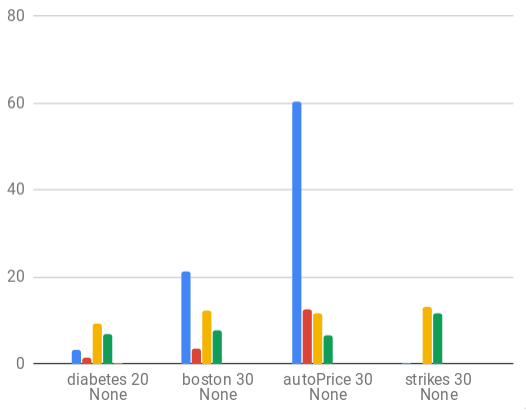
\includegraphics[width=0.5\textwidth]{time_easy.png} &
        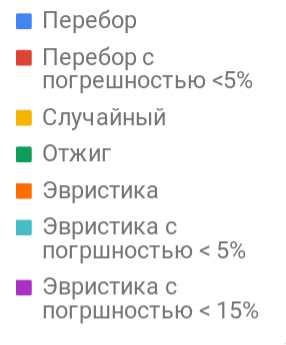
\includegraphics[width=0.3\textwidth]{time_legend.png} \\
        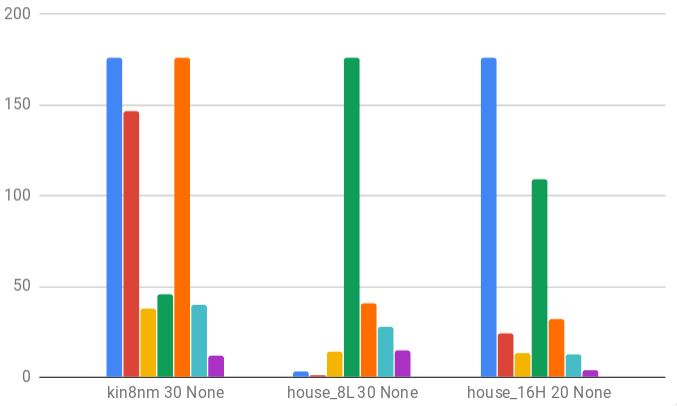
\includegraphics[width=0.5\textwidth]{time_big.png} &
        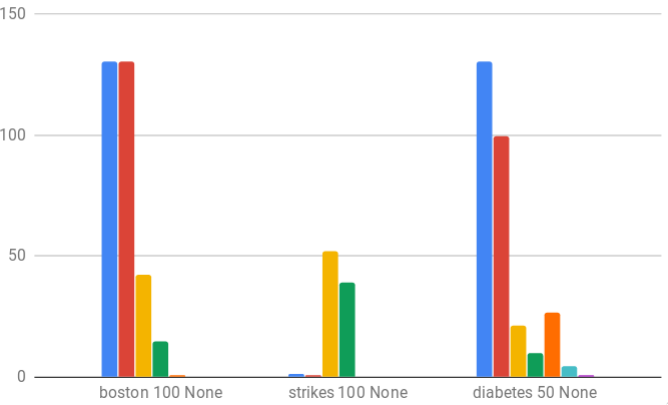
\includegraphics[width=0.5\textwidth]{time_trees.png} \\
    \end{tabular}
    \end{center}

    Как видно из графиков, время работы эвристического алгоритма оказывается
    всегда меньше других алгоритмов, особенно при допуске большой погрешности.

\subsection{Точность}
    \begin{center}
    \begin{tabular}{c c}
        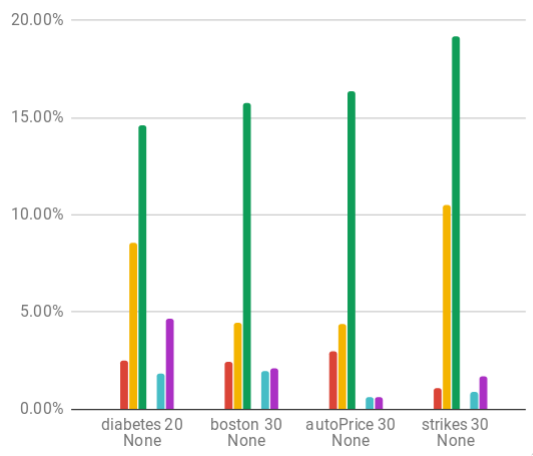
\includegraphics[width=0.5\textwidth]{error_easy.png} &
        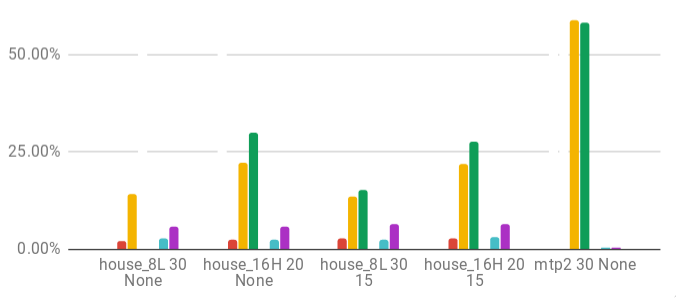
\includegraphics[width=0.5\textwidth]{error_features.png}
    \end{tabular}
    \end{center}

    Как видно из графиков, даже при большой погрешности эвристический алгоритм
    оказывается более точным нежели другие алгоритмы в сравнении.

\chapterconclusion{}

Эвристика демонстрирует лучшее время работы и при даже большой заданной погрешности 
находит результат более точный чем остальные алгоритмы. Текущая реализация
алгоритма имитации отжига не находит ответ точнее случайного алгоритма. Проблема
заключается в том, что большинство мутаций оказываются несущественными, так как
трешхолд находится в другом поддереве и не влияет на текущее значение.

%% Макрос для заключения. Совместим со старым стилевиком.
\conclusionpage{}

В данном разделе размещается заключение.

\printmainbibliography{}

\end{document}
